\documentclass[tikz,border=2pt]{standalone}
\usepackage{amsmath,amssymb}
\usepackage{tikz}
\usetikzlibrary{arrows.meta}

\begin{document}
% The sample standard deviation s = sqrt(s^2) is back in the units of the data: for the eight
% observations s = 2.0, and the band xbar +- s covers the "typical" observations.
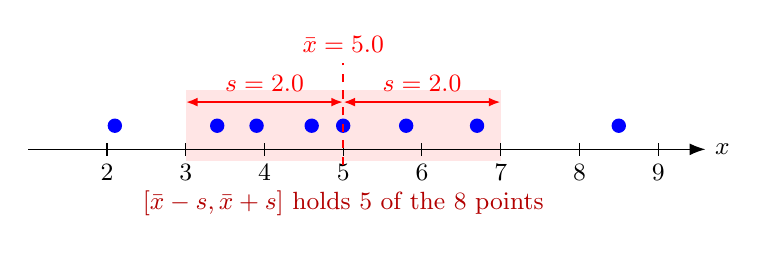
\begin{tikzpicture}[every node/.style={font=\small}, >={Latex[length=2mm]}]
	\fill[red!10] (3,-0.15) rectangle (7,0.75);
	\draw[->] (1,0) -- (9.6,0) node[right] {$x$};
	\foreach \x in {2,3,...,9} {\draw (\x,0.08) -- (\x,-0.08); \node[below=2pt, font=\small] at (\x,0) {\x};}
	\foreach \x in {2.1,3.4,3.9,4.6,5.0,5.8,6.7,8.5} {\fill[blue] (\x,0.3) circle (2.6pt);}
	\draw[red, dashed, thick] (5,-0.2) -- (5,1.1);
	\node[red, anchor=south] at (5,1.1) {$\bar x=5.0$};
	\draw[red, {Latex[length=1.5mm]}-{Latex[length=1.5mm]}, thick] (3,0.6) -- (5,0.6) node[midway, above, font=\small] {$s=2.0$};
	\draw[red, {Latex[length=1.5mm]}-{Latex[length=1.5mm]}, thick] (5,0.6) -- (7,0.6) node[midway, above, font=\small] {$s=2.0$};
	\node[red!70!black, font=\small, anchor=north] at (5,-0.4) {$[\bar x-s,\bar x+s]$ holds $5$ of the $8$ points};
	
\end{tikzpicture}
\end{document}
